\section{\texorpdfstring{Programování - Build}{Programovani - Build}}

% =====================================================================================================================
	\begin{frame}
    \frametitle{Build Pipeline}
		
		\begin{center}
			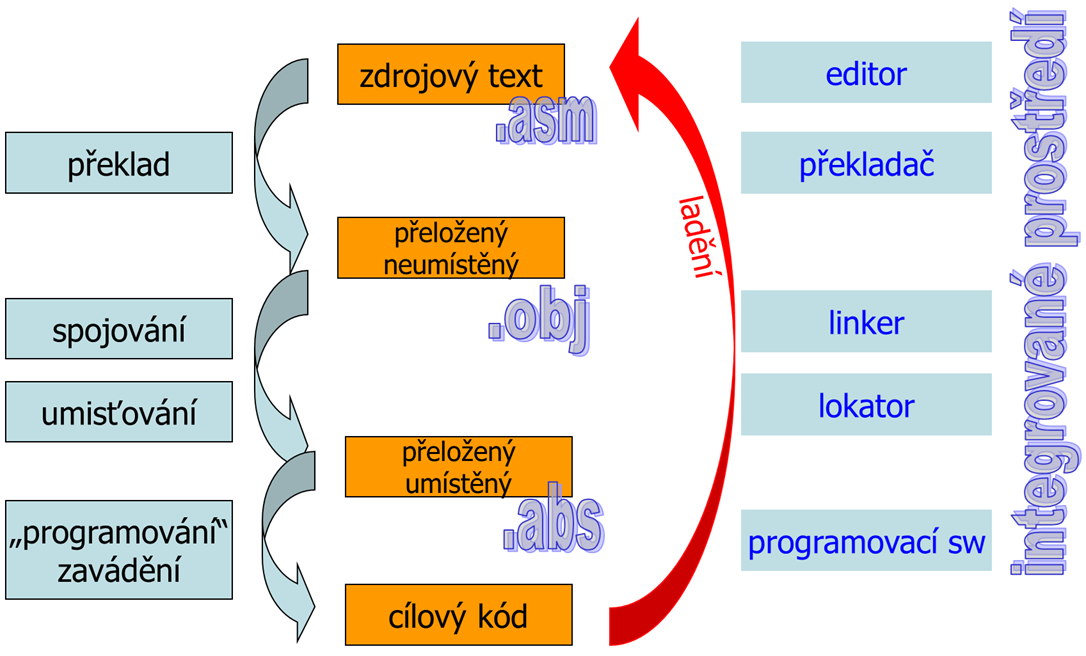
\includegraphics[width=1.00\textwidth]{fig/proces_programovani.png}
		\end{center}

	\end{frame}
	
% =====================================================================================================================
	\begin{frame}
    \frametitle{Zdrojový soubor}
		
		\begin{itemize}
			\item je kód, který píše programátor, tj. textový soubor,
			\item obsahuje popis proměnných, funkcí, skoků, logiky atd.,
			\item liší se podle programovacího jazyku = způsob popisu,
			
			\vspace{4mm}
			\item zdrojový soubor téhož programu psaný v assembleru se bude významně lišit mezi jednotlivými řadami procesorů - obvykle se liší jak v registrech tak v množině instrukcí,
			\item pro vyšší programovací jazyky (C, C++, ...) je podobnost zdrojového kódu vyšší - liší se hlavně v registrech a funkcích daného procesoru.
		\end{itemize}
	\end{frame}
		
% =====================================================================================================================
	\begin{frame}
    \frametitle{Překladač}
		
		\begin{itemize}
			\item Převádí zdrojový kód do strojově blízké formy - instrukce procesoru bez adres proměnných (tj. binární soubor),
			\item kontroluje chyby syntaxe jazyka, kontroluje typy proměnných apod.,
			\item generuje symboly:
			
			\begin{itemize}
				\item názvy funkcí,
				\item názvy proměnných,
			\end{itemize}
			
			\item výstupem je objektový soubor \textbf{\*.obj} (\textbf{\*.o}) pro každý zdrojový soubor.
		\end{itemize}
		
		\textbf{Příklad:}
		\begin{center}
			main.c $\longrightarrow$ main.o
			
			fibonacci.asm $\longrightarrow$ fibonacci.obj
		\end{center}
		
	\end{frame}
	
% =====================================================================================================================
	\begin{frame}
    \frametitle{Překladač STVD}
		
		\begin{center}
			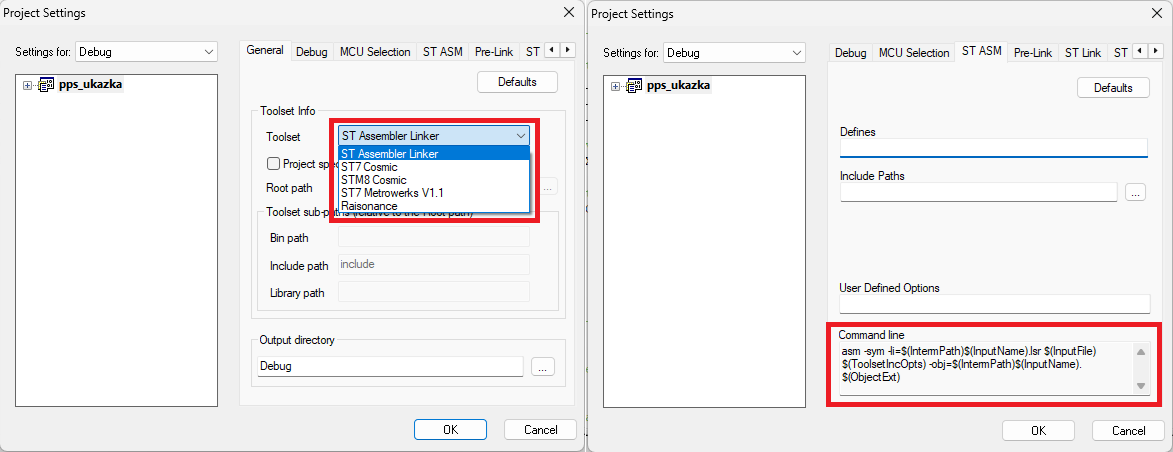
\includegraphics[width=1.00\textwidth]{fig/compiler.png}
		\end{center}

	\end{frame}
	
% =====================================================================================================================
	\begin{frame}
    \frametitle{Linker}
		
		\begin{itemize}
			\item Pracuje s celým projektem,
			\item spojuje jednotlivé objektové soubory a vyhrazuje jim adresy v paměti:
			
			\begin{itemize}
				\item adresy proměnných,
				\item adresy návěstí, ...
			\end{itemize}
			
			\item řeší také odkazy mezi soubory a do knihoven,
			
			\item výstupem je binární soubor \textbf{\*.hex} (nebo spustitelný soubor \textbf{\*.exe}) pro program.
		\end{itemize}
		
		\textbf{Příklad:}
		\begin{center}
			main.o, spi.o $\longrightarrow$ main.exe
		\end{center}
		
	\end{frame}
	
% =====================================================================================================================
	\begin{frame}
    \frametitle{Linker STVD}
		
		\begin{center}
			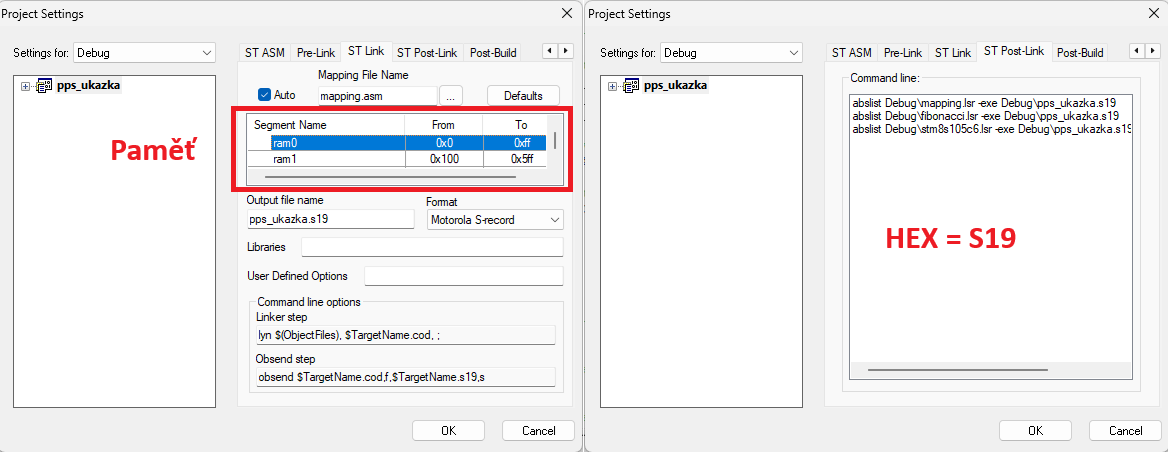
\includegraphics[width=1.00\textwidth]{fig/linker.png}
		\end{center}

	\end{frame}
	
% =====================================================================================================================
	\begin{frame}
    \frametitle{Výstupní hexfile typu MOTOROLA}
		
		\textbf{Program fibonacci.asm}
		\begin{center}
			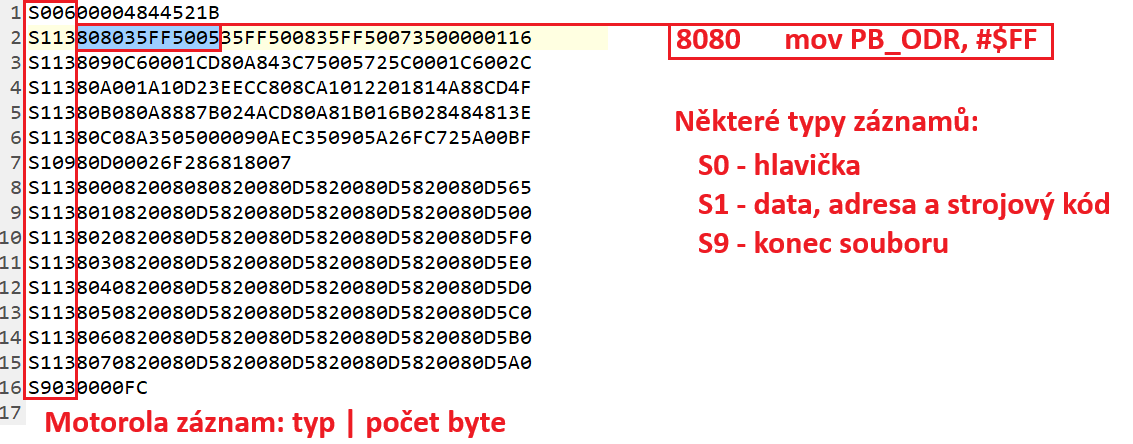
\includegraphics[width=1.00\textwidth]{fig/hexfile.png}
		\end{center}
		
		\begin{itemize}
			\item Zde je to textový soubor, nicméně může být také binární stejně jako objektové soubory.
		\end{itemize}

	\end{frame}